\documentclass[11pt]{article}

\usepackage{fullpage}
\usepackage{graphicx}

\begin{document}

\title{ARM11 - Final report}
\author{T. Tenev, E. Rossi, A. Spina, K. Ciszek}

\maketitle

\section{Assembler design}
When it came to designing the assembler, the first choice that needed to be made was whether to use a one pass or a two passes structure. We thought that this was a focal and key decision to all of the design, and thus we invested a considerable amount of hours working together to weight all the pros and cons of each different solution.

At first, we favoured the one pass approach (why using two passes when you can just use one?), but after careful reasoning we figured out that our implementation for it would have had a time complexity of $\mathcal{O}(n^2)$, with $n$ being the number of instructions in the assembly code; not to mention that it would have been much more tedious to code. Our idea consisted in using a hash table to map label names to addresses, then, when scanning the file instruction by instruction, if we should find a reference to a label (in a branch instruction), we would be in one of two situations: it is already been defined in the file or no definition has yet been given. In the first case we would just look up the corresponding address in the hash table, whereas in the second scenario we would add the given position to another hash table mapping labels to instructions that references the label (in case the label is not defined yet). Then, whenever a label definition is found, not only do we add the address of that label to the first hash table, but we also look at the list of instructions that reference that label in the second hash map, resolving those references.

This solution, although working, is considerably inefficient and more complex than the second one we considered: a simple two pass. The idea for the two pass is to start off as if we were considering a first pass (that is looking at all the label definitions in the code and filling a hash table that maps labels to addresses). Subsequently we would perform a second linear pass, and, as we know already the address of all the labels, we will encounter no forward references meaning that all the instructions could be resolved immediately.

Apart from being much easier to code, another advantage of this opportunity is its time complexity, which is just $\mathcal{O}(n)$; a lower bound for this kind of operation.
So, having considered the advantages and flaws of both designs, all together we opted to choose this second solution.

With this decision taken, the next choice regarded the in-detail implementation of this two pass.
An important design choice that we then made was to delegate all the reading of the assembly file to a single interface, "tokeniser.h"; an interface that could be used by both passes. The first pass thus used the tokeniser to get the label names and the relative addresses one by one, putting them for storage purposes into an hash table.

The second pass ended up being a bit more complicated, and therefore we created a central file that scans the input document using the tokeniser and, for every instruction, outsources the composition of the binary to a specific function. To do so we used a hash table that maps instruction names to functions, which are individual for each instruction (meaning that we have four of them). Using an hash table in this way allows us to avoid a a switch and gives us more flexibility.

\section{Extension}

\subsection{Summary}

Three additional modules were developed to complete the assembler tool kit, demonstrating a scenario which made use of the programs. A disassembler is a natural extension to the current system, enabling the conversion of binary executables into Assembler source code. BSI (Binary source image) is a wrapper of the PPM image format \cite{ppm} specially designed by us to represent executables as images which can be easily captured and processed to retrieve the binary source. Images produced by our BSI writer are used by a program running on the Raspberry Pi to execute binaries using paper as a storage device.

\subsection{Design}

\subsubsection{Disassembler}
A disassembler, by definition, is a program which translates a binary file into assembly code. Given the presence of pre-existent code used for our emulator and assembler sections, we chose a design consistent with what we already had. The actual functioning of the disassembler can be best described in the three following steps.

Firstly, using the already-implemented binary reader we load the data from the file into memory. The endianness is toggled and instructions can be fetched singularly using the tools built for the emulator. As we opted, similarly to the assembler, for a two-pass structure, during the first iteration we load address keys mapped to label values into a hash table for future reference.

Secondly, employing the present bit-field structs for the single instructions, we work our way "backwards" (if compared to the assembler) generating char* from integers. Where possible we use hash tables to lookup the strings given their corresponding key values. We also make use of assertions to make sure that the binary code we receive is well-formed.

Thirdly, having built the corresponding Strings to the instructions, we can now write them to the output file. We opted to test our disassembler indirectly; given assembly code we firstly assemble it into binary and subsequently disassemble it back into the original format. The relation between binary and disassembled code is bijective, but unfortunately such a connection does not hold between the assembler and disassembler, as multiple assembler codes could potentially result in the same binary.

\subsubsection{BSI writer}
The BSI writer program produces a PPM image from a binary file. Our current specification of the BSI format is quite simple and it is likely to undergo significant changes. The basic principle is best described with a sample image.

\begin{figure}[h]
\caption{BSI image format}
\centering

\includegraphics[scale=0.4]{images/gpio.jpeg}
\label{fig:bsi}
\end{figure}

Each string of white and black blocks represents a memory word. A high-contrast background is used to aid processing of printed images. In fact the image above is the BSI representation of our Assembler program from Part III.

\subsubsection{BSI capture and execution}
The idea to use paper as a storage device for our executables was inspired by our broken SD card adapter. Disappointed by unreliable hardware, we decided to look back in the history of computing seeking for an alternative means of storage as a backup. On a more serious note, we wanted to explore image processing algorithms and their performance when running C on a Raspberry Pi.

A minimal image processing library \cite{imgproc} which provides useful APIs for interacting with a camera and displaying and processing images is used for developing a BSI scanner. Basic colour filtering and edge detection algorithms are used to convert the captured frames into a binary. Capture continues until a working binary is constructed which can then be executed on the Raspberry Pi.


\section{Testing}
\subsection{Unit Testing}
All the members have been using unit testing right from the start of the implementation and a minimal approach was adopted. This enforced the existence of self-contained testable modules that could be reused and changed reliably. It has also turned out to be essential to find bugs as soon as possible and avoiding their propagation in the project.
To simplify testing, we set up a make target that allows us to run all the tests every time we compile the project. 

\subsection{Continuous Integration}
Continuous integration was configured on Gitlab to build the make targets and run all tests on each push to all remote branches. This was the best way to be 100\% sure that all the commits to our main working branch (develop) were passing our tests. You can see a screenshot from our Gitlab in figure \ref{fig:ContInt}.

\begin{figure}[h]
\caption{Screenshot from our Gitlab Continuous Integration}
\centering
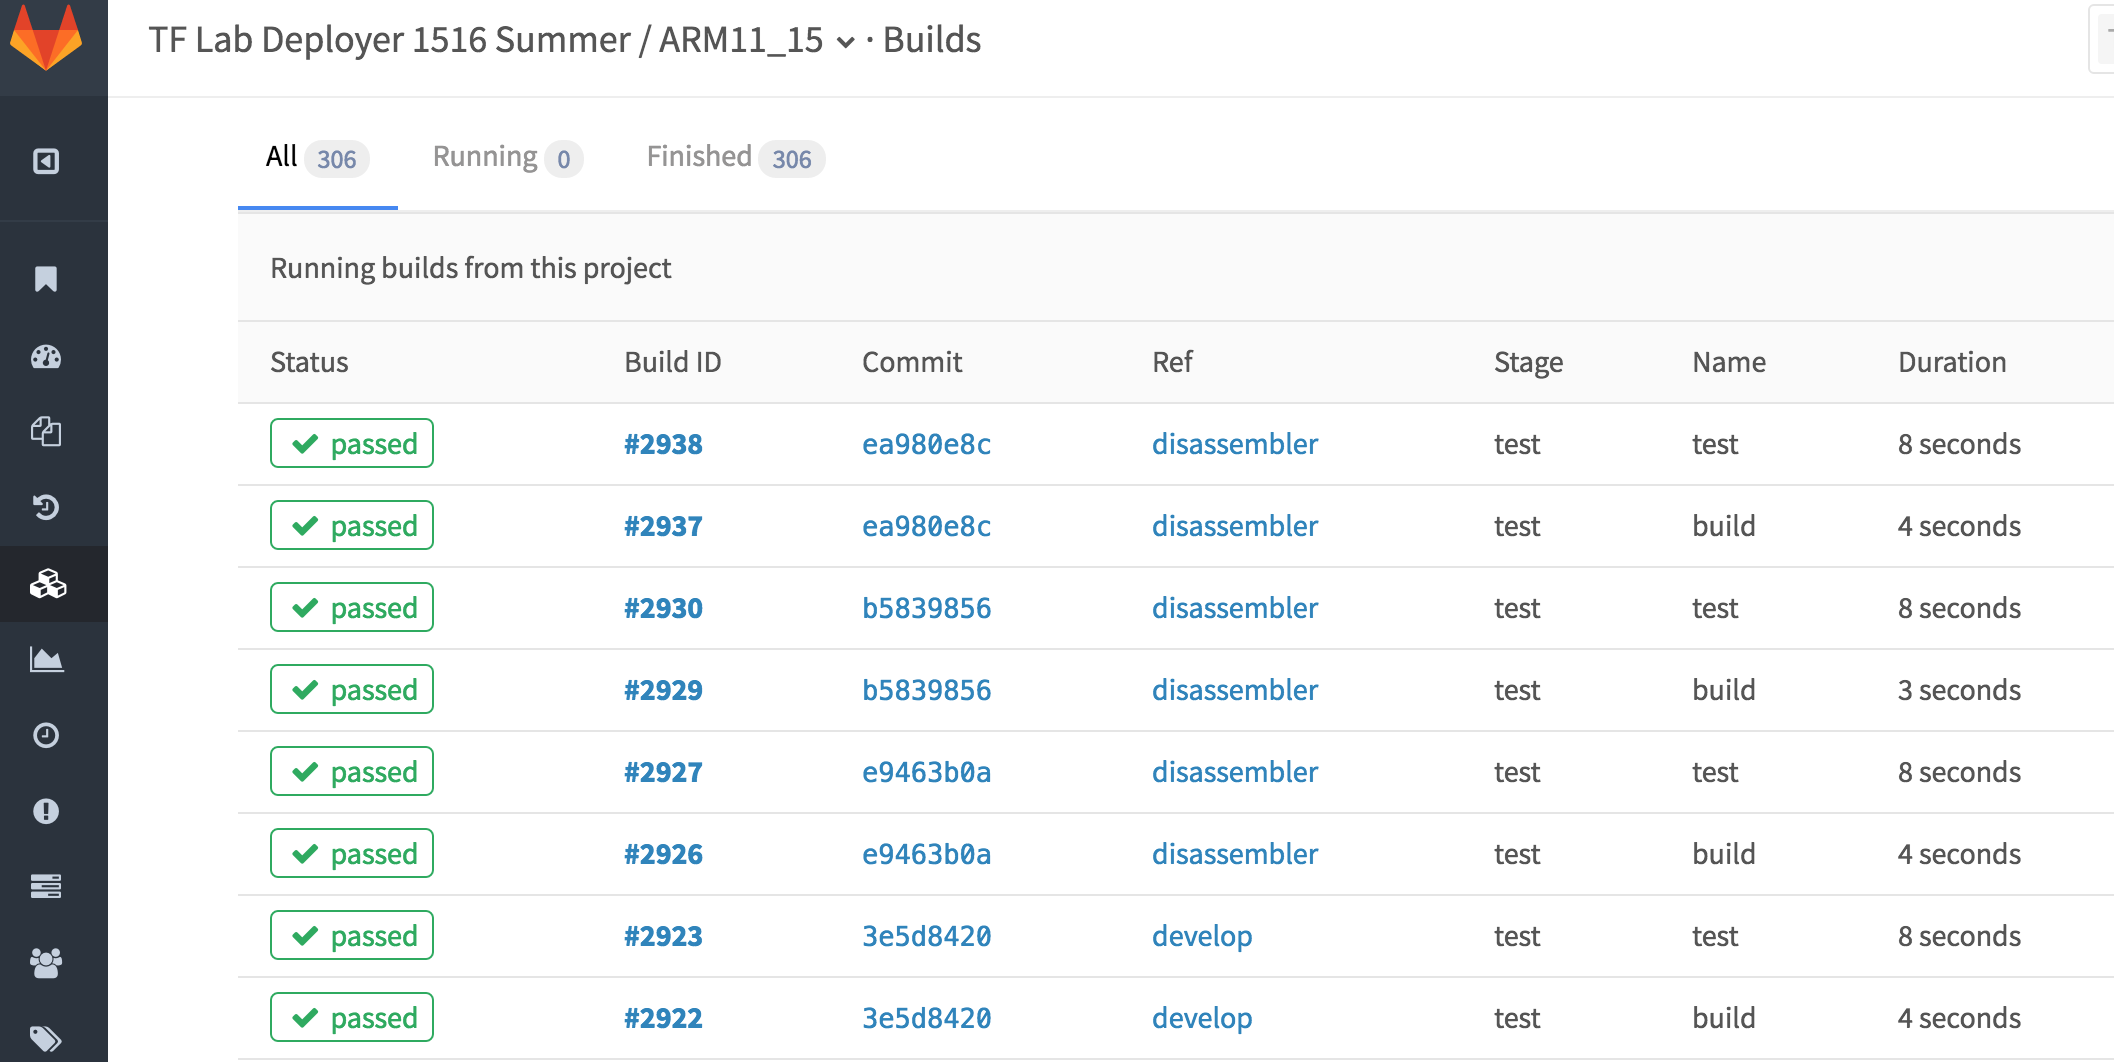
\includegraphics[width=0.8\textwidth]{images/ContInt}
\label{fig:ContInt}
\end{figure}

\subsection{Provided Test Suite}
When we implemented all features in our assembler, we started testing it against the provided test suite. This testing has proved to be invaluable to find subtle bugs (such as overflow in certain cases of binary subtraction). We adopted a regression testing approach, that is committing to our working branch only after having checked that the tests passed by the commit prior to our version were also, at least, passing in our current code.

\section{Group reflection}
 
\subsection{Group improvement}
It was amazing to see all of us get better day after day. We all agree that most of this improvement comes from the collaboration we have enjoyed throughout the whole project. Using merge requests meant that each line of code was verified by at least two team members. These code reviews allowed us to learn from each other and to share our opinion on different ways of solving the same problem.

\subsection{Overcoming difficulties}
Another important part of our teamwork was that not only didn't difficulties tear us apart, but instead they strengthened us increasing the bonds and connections between each other. In particular, once, after a long and tiring day we had a little argument between two members about the approach that was being taken, but we immediately realised that such issue was caused by a temporary lack of communication of the team. We thus decided to meet all together the following morning to talk explicitly about those problems and to solve them together. This was by far the best solution, that allowed us to continue the project without resentment and improved our communication. 

\subsection{Sharing decisions}
Instead of delegating different parts to different people, and assigning them the design of each part, we thought it was of prior importance to take all the important design decisions together. We would break up bigger implementations into smaller problems assigned to single group members; in such a way we constantly had different opinions and could make the best choice every time. We applied such principle to the emulator, where it resulted in a very interesting design for the structure of the memory, and to the assembler, where we obtained very stimulating discussions that lead us to our two passes solution.

\subsection{Handling unexpected situations}
Between all the challenges we were expecting to face, having long lasting health problems was not in the list. Therefore, when one member was hospitalised for two weeks, it meant we had to reorganise our plan and redistribute among the rest the amount of work. In the end we successfully handled this situation, by asking frequent updates on the situation of the hospitalised member and making sure his absence was influencing the result of the project as little as possible.

\section{Individual reflections}

\subsection{Tencho Tenev}
The project has taught me that, while most aspects of software implementation can be planned and designed to the slightest detail, the more general project development process is much more challenging in terms of organisation. I learnt to give and rely on estimates, to negotiate and design pre and post-conditions, and to modify existing plans in response to changes in the design, group dynamics and requirements. Spending 3 days debugging an issue with our implementation of Part III was the biggest challenge for me, maybe because it turned out to be a hardware problem. Overall, I am very satisfied by the group experience during the last weeks.

\subsection{Emanuele Rossi}
From the start I knew that this experience would be a great challenge, mainly because it was my first big project in group, and even if I had done something of similar size on my own in the past, working in group requires an additional set of skills. 
Still, I wasn't scared of it, and I was actually looking forward to it, willing to learn as much as possible. Overall, I think that being the team leader ended up being the perfect opportunity. 
Right from the start I knew that my responsibility was as much developing the project as making sure that the communication and the relationships between the group members were the best they could be.

Regarding WebPAs, even if I regard them as important, I preferred to ask for "face to face" feedback continuously during the project, as I strongly believe that other people's opinions make us notice possible improvement that we could not even think of on our own. From those feedback I learnt how to be as helpful as possible to my team mates and how to communicate efficiently with them.

To conclude, I am convinced that this experience has been as much a programming experience for me as a social experience. And I think that all the skills that this project taught me make me a better person and give me the confidence I needed for the internship I am going to undertake this summer.

\subsection{Alberto Spina}
Throughout my short "career" as a computer scientist, I have always been fascinated and intrigued by machine language, and I believe that the depth, and maybe overall complexity, of this project has enabled me to explore and understand thoroughly such a passion of mine. I knew I would have been up against a demanding task, but the constant presence of a group to back me up made the overall experience more than enjoyable.

I am aware that I lack in confidence when coding, and such a belief of mine seems to be supported by a never-ending streak of compile errors. But the presence of fellow students around me gave me confidence and got me started; I began slowly, but soon became passionate over the topic; maybe a bit overly excited, as WebPA feedback made me realise. My stubbornness hasn't been eradicated completely, as I would still give myself daily goals and commit to completing them in time, and I appreciate that it enables me to meet deadlines on time. 

I strongly believe that this has been the finest and most thorough group experience I have ever had. There is no task that we haven't split among all members, and this procedure of ours required extensive amounts of teamwork and communication. But when, as it has happened, we realised that our overall group participation was leaking, we came back together as a whole overcoming any difficulties we might have encountered.

\subsection{Karol Ciszek}
For me, the project has been a great experience, but not for the reasons that I would have imagined. There has been a lot of personal progress on my part, both in terms of coding ability, as well as communication skills and programming in a group. It was very satisfying to see each member (myself included) adapt to suit both the group's needs according to their own strengths.

It is important to note that I have been hospitalised for two weeks during the bulk of the project. This brought up my main personal challenge for the project: communication with the rest of the group during this time, as the team, of course, needed to know what is going on in my personal life. However, in order to remain relatively professional during the course of the project, I needed to keep my personal life separate from the work; hence, my communication skills were put thoroughly to the test.

The most important lesson I learnt, is that personal issues in group work must not be hidden. As difficult as it might be to admit that something is wrong, being clear in expressing what exactly is happening will allow the group to overcome obstacles as a whole.
\medskip

\begin{thebibliography}{1}

\bibitem{imgproc}
Jones, E.
\textit{http://www.cl.cam.ac.uk/downloads/freshers/image\_processing.tar.gz}

\bibitem{ppm}
Netpbm
\textit{http://netpbm.sourceforge.net/doc/ppm.html}

\end{thebibliography}

\end{document}

